\documentclass[12pt]{article}
\usepackage{geometry}
\usepackage{graphicx}
\usepackage{amsmath}
\usepackage{enumitem}
\usepackage{parskip}
\usepackage{setspace}
\usepackage{float}
\usepackage{relsize}
\usepackage{listings}
\usepackage{fancyvrb}
\AtBeginEnvironment{align}{\setcounter{equation}{0}}
\allowdisplaybreak

\onehalfspacing
\geometry{letterpaper, portrait, margin=1in}

\newcommand{\qnot}{\scalebox{.8}{$\mathrm{NOT}$}}
\newcommand{\qI}{\scalebox{1}{$\mathrm{I}$}}

\newcommand{\dsum}[2]{\mathlarger{\sum}_{#1}^{#2}}
\newcommand{\bgc}{\begin{center}}
\newcommand{\enc}{\end{center}}
\newcommand{\Lg}{\mathcal{L}}
\newcommand{\norm}[1]{\left\lVert#1\right\rVert}
\newcommand{\colvs}[1]{\begin{bsmallmatrix} #1 \end{bsmallmatrix}}
\newcommand{\colv}[1]{\begin{bmatrix} #1 \end{bmatrix}}
\renewcommand{\arraystretch}{.8}
\newcommand{\state}[1]{\left| #1 \right \rangle}
\newcommand{\tran}{\mathsf{T}}
\newcommand{\sotimes}{\scalebox{.9}{$\otimes$}}
\newcommand{\rarrowtext}[1]{\xrightarrow{\mathrm{#1}}}



\begin{document}
\noindent CSCI 4962 \hfill Project Report \\
Siddha Kilaru \\

\bgc
\textbf{Neural Networks as Numeric Solvers}
\enc

\begin{description}
    \item[Introduction] \hfill \\
    The goal of this project is to explore how neural networks can be used to
    approximate solutions to differential equations. The paper ``Physics
    Informed Deep Learning'' by Maziar Raissi, Paris Perdikaris, George Em
    Karniadakis is the inspiration for this project. The paper introduces the
    concept of physics-informed neural networks and uses it to find solutions
    to nonlinear partial differential equations. In this project, I use the
    methods detailed in the paper but with simpler differential equations.
    Specifically, I focus on first-order and second-order ordinary differential
    equations (ODE), which have analytical solutions. In reality, there is no
    use in approximating a differential equation with an analytical solution;
    however, for the purposes of this project, I want to compute the accuracy
    of the approximated solution. In addition to using the methods outlined in
    the paper, I also experiment with different model hyperparameters and see
    how it affects the runtime and accuracy. Finally, I compare approximate
    solutions derived from neural networks with traditional methods such as
    Euler's and higher-order Runge-Kutta methods.

    \item[Unsupervised Approach] \hfill \\
    Consider the simple differential equation $y' = x$ with initial condition
    $y(0) = 1$. Also, assume we use a neural network to approximate the
    solution in a supervised learning setting. The set of features would be the
    $x$ points, but the set of labels is not immediately obvious. One could say
    the set of labels is a finite set of $y$ points. There are a couple of
    problems, however. First, if the differential equation has no solution,
    then the labels are unattainable. Secondly, if we use real-world, observed
    data, it might be too granular and contain too much noise. As a result, a
    supervised learning model is not completely appropriate for this task. The
    paper mentioned above uses an alternative method that makes use of
    unsupervised learning. The main idea is for the neural networks to learn
    the gradient of the differential equation. Moreover, for a given set of
    labels containing $x$ points, each $x$ point replicates the gradient
    described by the differential equation. In the case of $y' = x$, the
    gradient at each point should be equal to $x$. One way to do this is by
    devising an error function as follows: 
    \bgc 
    $\alpha\Bigl(\dsum{i-0}{n}(\hat{y}_i' - x_i)^2\Bigr)^{1/2} + \beta(\hat{y}_0 - 1)$.
    \enc
    Above, $\alpha$ and $\beta$ are hyperparameters. The first term in the sum
    enforces the ODE constraint, and the second term enforces the initial
    condition. A neural network can use this error function to find an
    approximate solution. I experiment with different differential equations
    and their corresponding error functions in the sections below. 

    \item[Approximating First Order ODEs] \hfill \\
    First, let us consider the differential equation $y' = e^x$ with initial
    condition $y(0) = 1$. Trivially, the solution can be analytically
    determined to be $y = e^x$. To approximate the solution, a neural network
    with three hidden layers will be used. One of the hyperparameters for the
    model is the depth of each hidden layer, $d$. The other two hyperparameters
    $\alpha$ and $\beta$ are part of the loss function:
    \bgc 
    $\alpha\Bigl(\dsum{i-0}{n}(\hat{y}_i' -e^{x_i})^2\Bigr)^{1/2} + \beta(\hat{y}_0 - 1)$.
    \enc
    To find the optimal $\beta$, I fix $\alpha = 1$, $d = 20$, and do a search with
    $\beta\in[0, 20]$. The results of the grid search are shown in the plot
    below.\\
    \begin{minipage}{\linewidth}
        \centering
        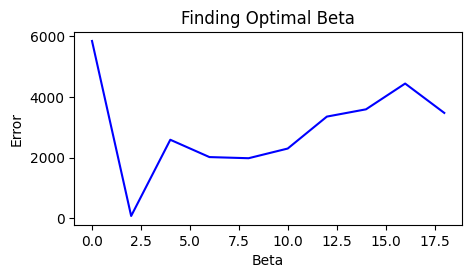
\includegraphics[scale=.5]{images/figure1.png}
    \end{minipage}
    In the plot, the x-axis represents the different $\beta$, and the y-axis is
    the error defined as 
    \bgc 
    $\dfrac{1}{n}\dsum{i=0}{n}(\hat{y}_i - y_i)^2$.
    \enc
    The minimum error occurs when $\beta = 2$, which is the estimated optimal
    value. Next, after training the model, the following results were achieved: \\
    \begin{minipage}{\linewidth}
        \centering
        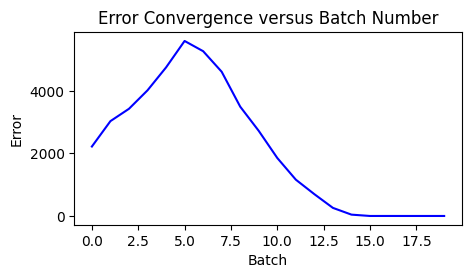
\includegraphics[scale=.5]{images/figure2.png}
    \end{minipage}
    As you can see in the plot above, the error started to decrease rapidly
    just after a few batches. Also, looking at the plots below, the approximate
    solution very closely matches the exact solution. \\
    \begin{minipage}{\linewidth}
        \centering
        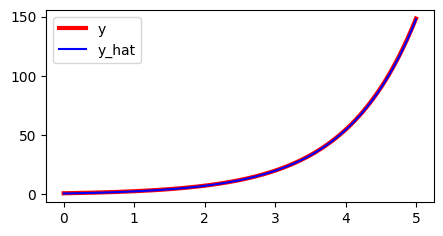
\includegraphics[scale=.5]{images/figure3.png}
        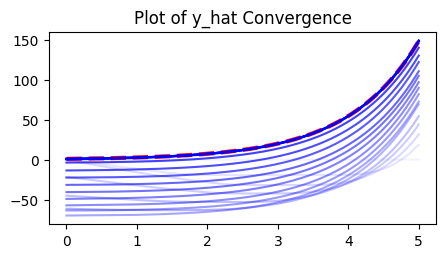
\includegraphics[scale=.5]{images/figure4.png}
    \end{minipage}
    \hfill \\
    \hline
    \hfill \\
    Moving on, we now focus on the differential equation $5y' - 4y^2 = 0$ with
    initial condition $y(0) = -8$; the exact solution is $-\frac{40}{32x+5}$.
    The loss function is 
    \bgc 
    $\alpha\Bigl(\dsum{i-0}{n}(5\hat{y}_i' - 4\hat{y}_i^2)^2\Bigr)^{1/2} + \beta(\hat{y}_0 + 8)$.
    \enc
    I find the optimal $\beta = 11$ and $\alpha=1$. Now, I focus on how the
    depth of the neural network affects accuracy and runtime. For $d\in[20,
    500]$, I get the plot below.  \\ 
    \begin{minipage}{\linewidth}
        \centering
        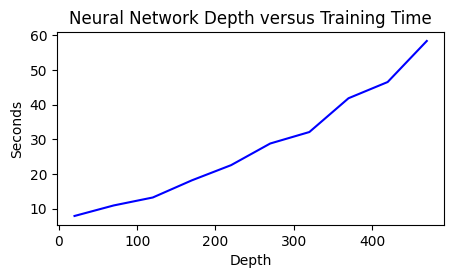
\includegraphics[scale=.5]{images/figure5.png}
        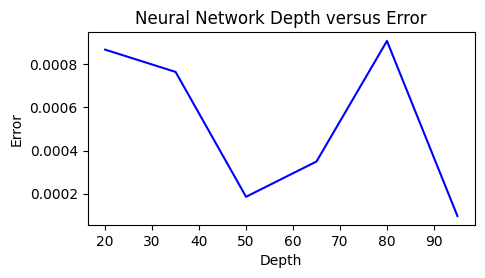
\includegraphics[scale=.5]{images/figure6.png}
    \end{minipage}
    Looking at the plot, there is a clear relationship between depth and
    training time: as the depth increases, the training time increases. The
    relationship appears linear in the plot; however, more investigation is
    needed to determine if that is actually the case. According to the second
    plot, the optimal depth is 95; however, 50 also yields a very low error. If
    we also consider the run time in choosing the optimal depth, then perhaps
    50 is better because of its shorter runtime. Finally, looking at the plots
    below, we can see that the approximate solution is very close to the exact
    solution. \\
    \begin{minipage}{\linewidth}
        \centering
        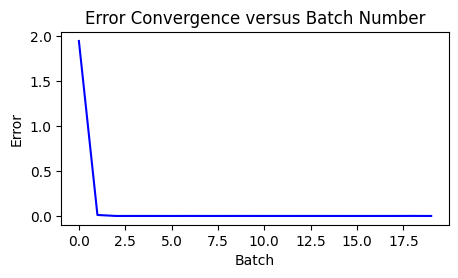
\includegraphics[scale=.5]{images/figure7.png}
        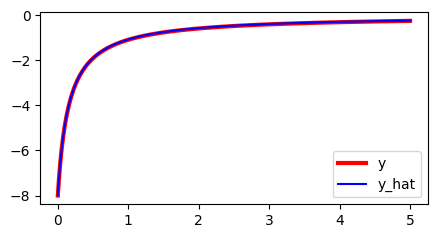
\includegraphics[scale=.5]{images/figure8.png}
    \end{minipage}

    \item[Approximating Second Order ODEs] \hfill \\
    Now, let us experiment with the second order differential equation $10y''+
    5y = 0$ with initial conditions  $y(0) = 0$ and $y'(0) = 1$; the exact
    solution is $\sqrt{2}\sin(\frac{x}{\sqrt{2}})$. The loss function is 
    \bgc 
    $\alpha\Bigl(\dsum{i-0}{n}(10\hat{y}_i'' + 5\hat{y}_i)^2\Bigr)^{1/2} 
    + \beta(\hat{y}_0)
    + \gamma(\hat{y}_0' - 1)$.
    \enc
    Note that compared to the first order, there is an extra term due to the
    added initial condition. Moving on, I find the optimal $\alpha = 1$, $\beta
    = 1$, and $\gamma = 500$ using the same method. These are the results
    for $x\in[0, 20]$: \\
    \begin{minipage}{\linewidth}
        \centering
        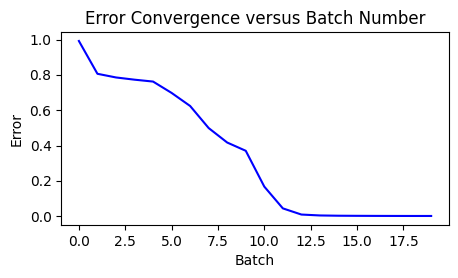
\includegraphics[scale=.5]{images/figure9.png}
    \end{minipage}
    As you can see above, the error decreases significantly towards zero.
    Moreover, looking at the plots below, the approximate solution matches the
    exact solution very closely. \\
    \begin{minipage}{\linewidth}
        \centering
        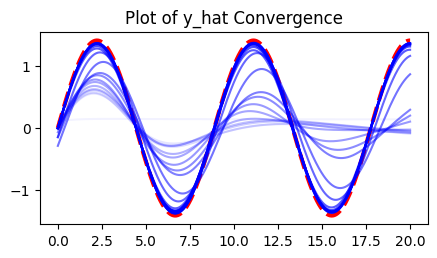
\includegraphics[scale=.5]{images/figure10.png}
        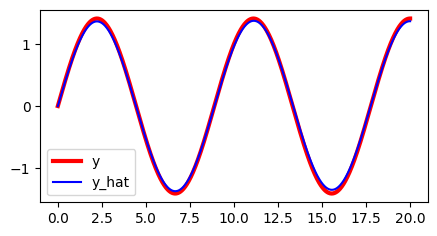
\includegraphics[scale=.5]{images/figure11.png}
    \end{minipage}
    The results shown above are very promising however, what does the
    approximate solution look like outside the domain $x\in[0, 20]$ of which
    the neural network was trained on? Looking at the plot below, we can see
    that approximate solution starts to diverge away from the exact solution.
    This kind of behavior is expected because since we only train the neural
    network on a specific range of $x$ values, only those values should have
    the correct gradient. In other words, the model does not prioritize
    generalization at all; instead, the model focuses on approximating as close
    as possible to the desired solution. \\
    \begin{minipage}{\linewidth}
        \centering
        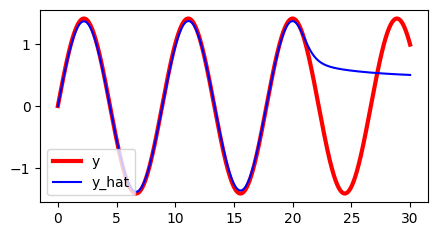
\includegraphics[scale=.5]{images/figure12.png}
    \end{minipage}
    \hfill \\
    \hline
    \hfill \\
    Similar to the last differential equation consider $my'' + by' + ky = 0$.
    In physics, this equation models damped oscillatory behavior, or in other
    words, a damped spring. Let us set $m = 10$, $b = 2$, and $k = 2$. Here the
    mass is $2$, damping constant is $2$, and spring constant is $2$.  Also,
    let the initial conditions be $y(0) = -10$ and $y(0)' = 0$. These
    conditions state that the object starts at position $-10$ with $0$ initial
    velocity. The exact solution to this is 
    \bgc 
    $y(x) = -\dfrac{10}{19} e^{-\frac{x}{10}} (\sqrt{19}\sin(\sqrt{19}x/10) + 19\cos(\sqrt{19}x/10))$,
    \enc
    and the loss function is 
    \bgc 
    $\alpha\Bigl(\dsum{i-0}{n}(10\hat{y}_i'' + 2\hat{y}_i' + 2\hat{y}_i)^2\Bigr)^{1/2} 
    + \beta(\hat{y}_0 + 10)
    + \gamma(\hat{y}_0')$.
    \enc
    Training the neural network with $x\in[0, 55]$ with $50$ points yields the
    results below. \\ 
    \begin{minipage}{\linewidth}
        \centering
        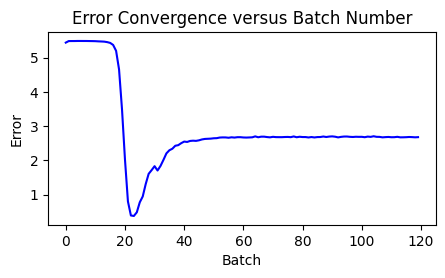
\includegraphics[scale=.5]{images/figure13.png}
        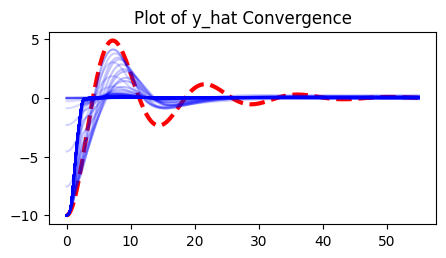
\includegraphics[scale=.5]{images/figure14.png}
    \end{minipage}
    Interestingly, the error rapidly decreases then starts to increase. This is
    also represented in the second plot where it first starts to properly fit,
    then starts reverting into a worse approximation. I theorize this is due to
    the fact that 50 points in the range 0 to 55 is not enough. The fewer
    points cause a single point to appease to contrasting gradients. Below are
    the results for the neural network trained with $x\in[0, 55]$ with $300$
    points. \\
    \begin{minipage}{\linewidth}
        \centering
        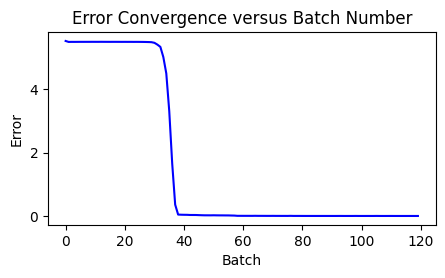
\includegraphics[scale=.5]{images/figure15.png}
        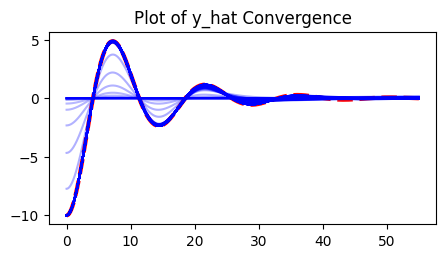
\includegraphics[scale=.5]{images/figure16.png}
    \end{minipage}
    Now, the error function is monotonically decreasing, and the approximate
    solution is very close to the exact solution. Another interesting thing
    about this solution in particular is that it decays, or in other words the
    derivative flattens as $x$ increases. A consequence of this is that unlike
    the previous equation where the approximate solution deviates away from the
    exact solution, the approximate solution will continue to follow the exact
    solution. This can be seen in the plot below. The network was only trained
    for $x\in[0, 50]$, but the plot is for $x\in[0, 150]$. \\
    \begin{minipage}{\linewidth}
        \centering
        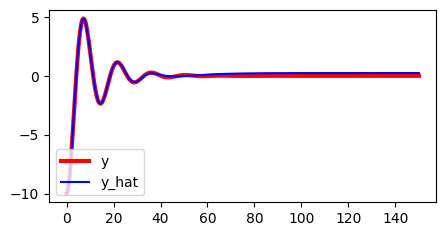
\includegraphics[scale=.5]{images/figure17.png}
    \end{minipage}
    \item[Comparison to Traditional Methods] \hfill \\
\end{description}


\end{document}